\section{Single Phase Half Wave Controlled Rectifier with RLE load}

\subsection{Circuit used for simulation}

% figure that is centered on the page
\begin{figure}[h]
    \centering
    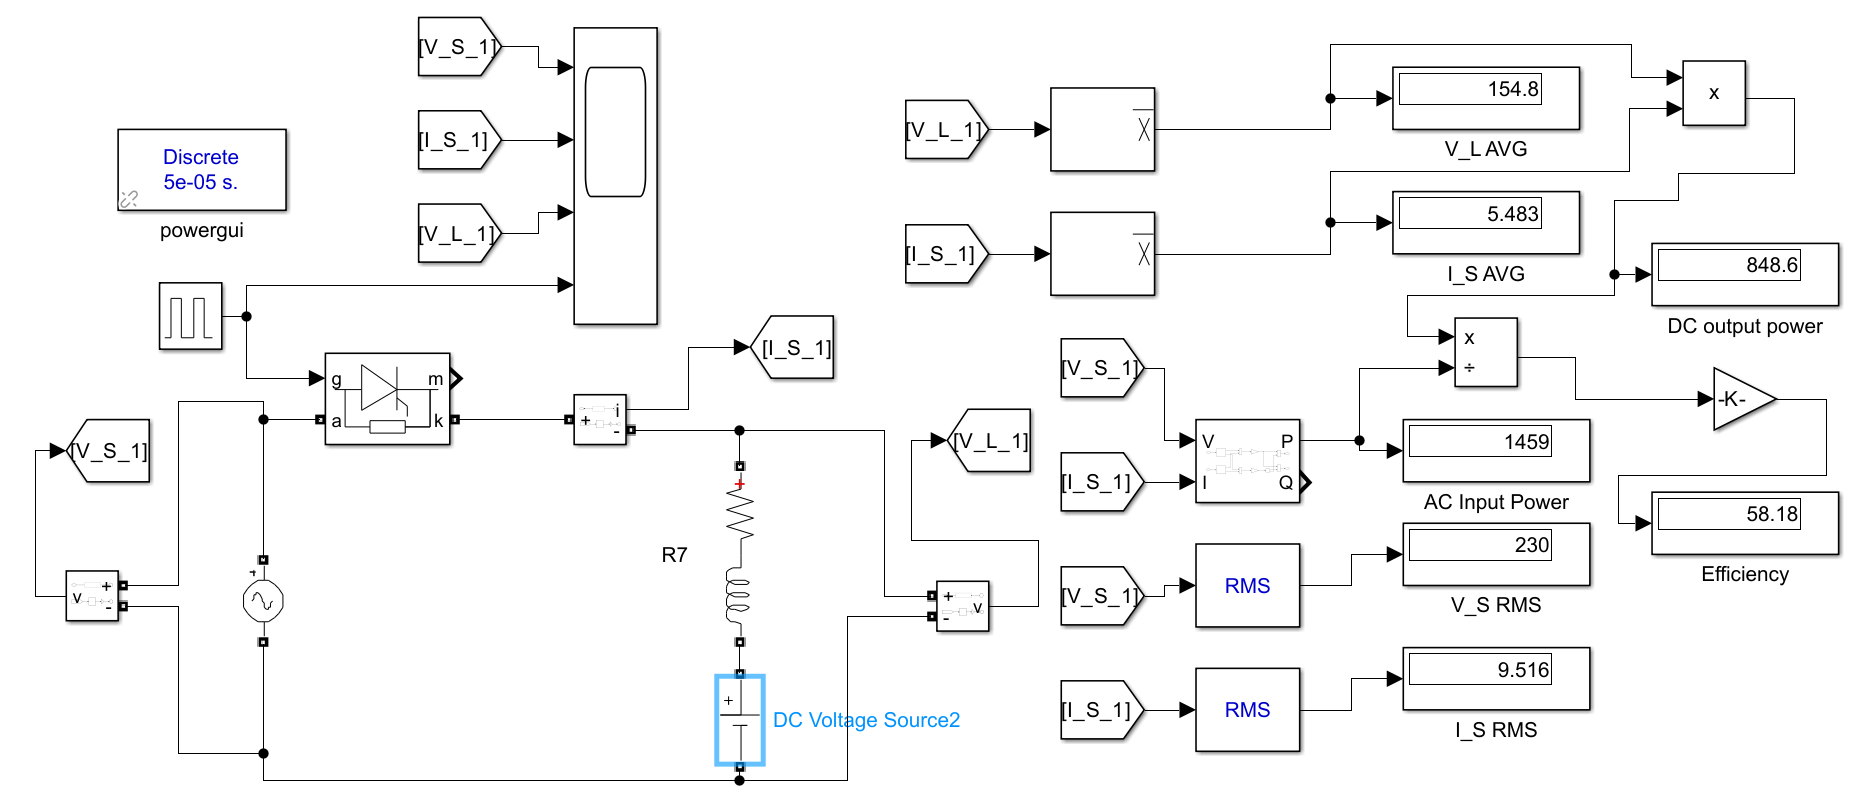
\includegraphics[width=1.0\textwidth]{images/experiment-1/circuit-diagram-experiment-07.png}
    \caption{Circuit for Single Phase Half Wave Controlled Rectifier with RLE load (Firing Angle = 30$ ^\circ $)}
    \label{Fig_simulation_circuit_single-phase-half-wave-controlled-rectifier-with-RLE-load}
\end{figure}

\subsection{Components Required}

\begin{table}[h]
    \renewcommand{\arraystretch}{1.3}
    \label{table_components_required_single-phase-half-wave-controlled-rectifier-with-RLE-load}
    \centering
    \begin{tabular}{|c|c|c|c|}
        \hline
        Sr. No & Parameters                     & Ratings            & Quantity \\
        \hline
        \hline
        1      & AC Single Phase Voltage Source & 230V ($ V_{rms} $) & 1        \\
        \hline
        2      & Resistor                       & 10$ \Omega $       & 1        \\
        \hline
        3      & Inductor                       & 10mH               & 1        \\
        \hline
        4      & Diode                          & -                  & 1        \\
        \hline
        5      & Voltmeter                      & -                  & 2        \\
        \hline
        6      & Ammeter                        & -                  & 1        \\
        \hline
        7      & Thyristor                      & -                  & 1        \\
        \hline
        8      & DC Source                      & 100V               & 1        \\
        \hline
    \end{tabular}
    \caption{Components for Single Phase Half Wave Controlled Rectifier with RLE load}

\end{table}

\pagebreak

\subsection{Observations}

\begin{table}[h]
    \renewcommand{\arraystretch}{1.3}
    \label{table_observation_single-phase-half-wave-controlled-rectifier-with-RLE-load}
    \centering
    \begin{tabular}{|c|c|c|}
        \hline
        Parameters                              & Theoretical Values & Simulation Values \\
        \hline
        \hline
        AC Input Voltage ($ V_{in,rms} $)       & 230V               & 230V              \\
        \hline
        Output Average Voltage ($ V_{o,avg} $)  & 96.66V             & 155.1V            \\
        \hline
        Output Average Current ($ I_{o,avg}  $) & 9.66A              & 5.507A            \\
        \hline
    \end{tabular}
    \caption{Observations for Single Phase Half Wave Controlled Rectifier with RLE load}

\end{table}


Upon giving the firing gate pulse to the thyristor, the circuit is observed to initiate conduction. Once the circuit initiates conduction, its characteristics resemble those of an uncontrolled half wave rectifier with RLE load.
Additionally, the DC output power was estimated to be 848.6W, while the AC input power was found to be 1459W, resulting in an overall efficiency of 58.18\%.




% \pagebreak


\subsection{Resultant Waveforms}

% figure that is centered on the page
\begin{figure}[h]
    \centering
    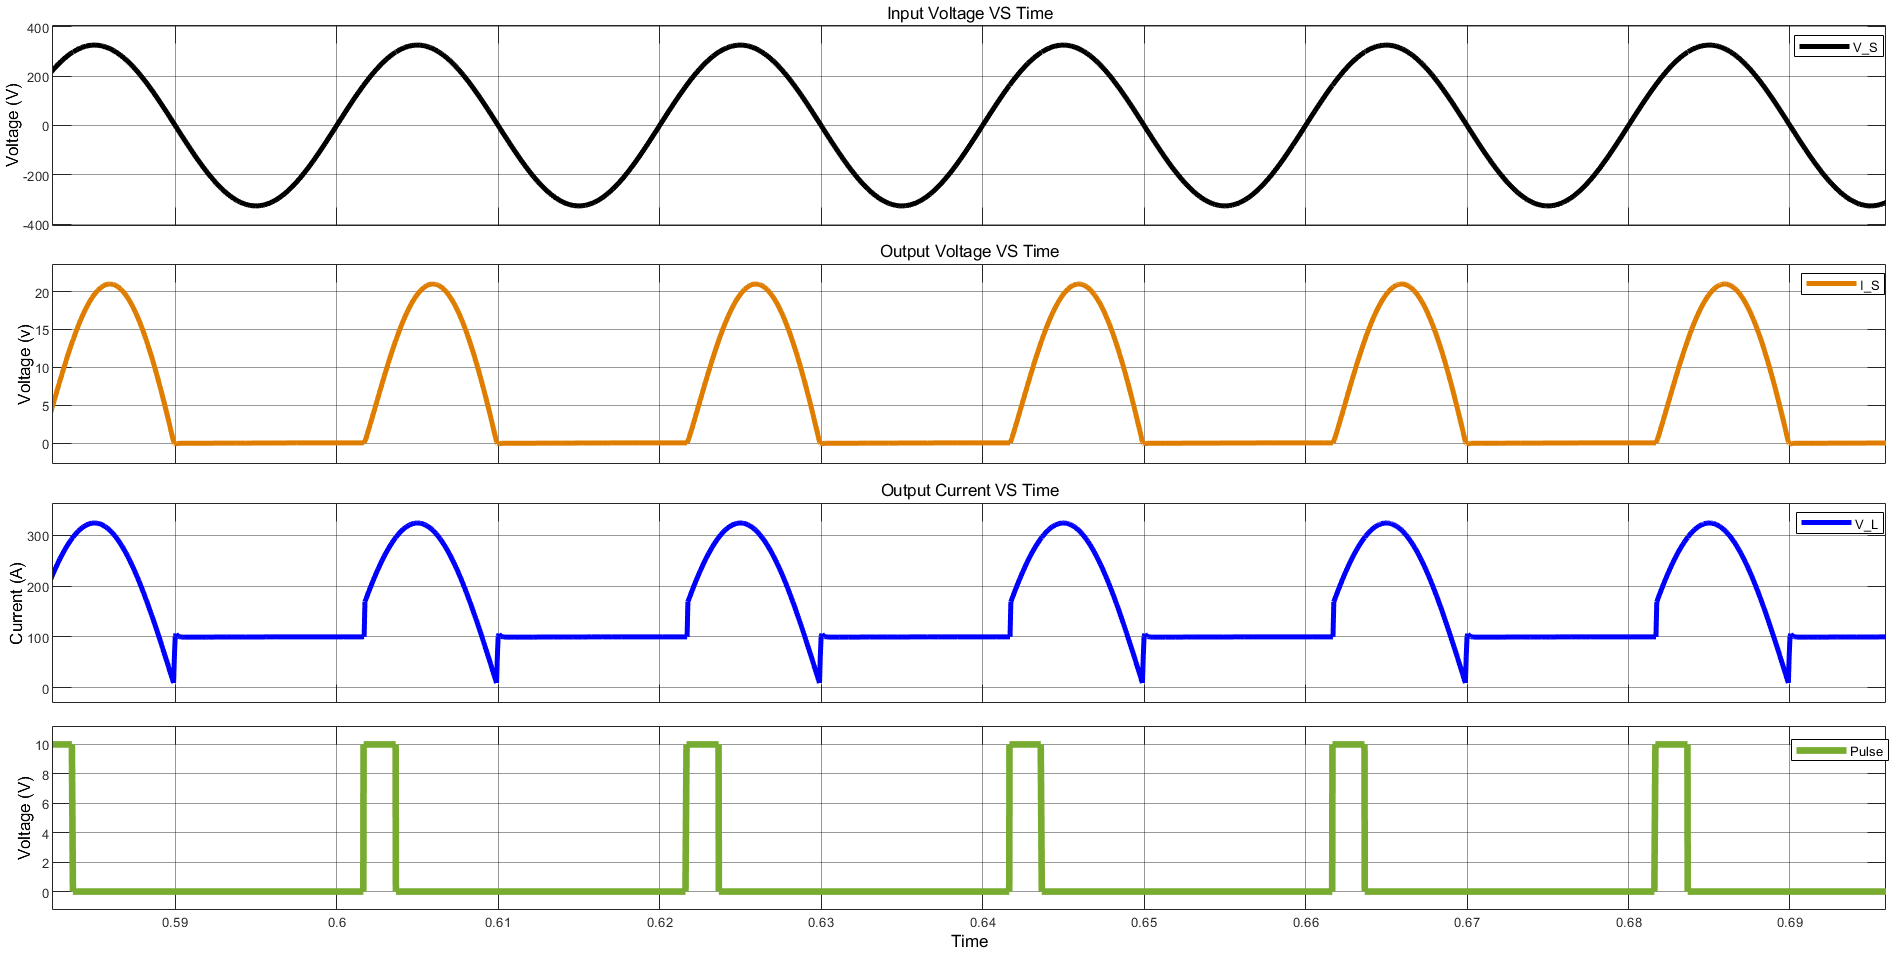
\includegraphics[width=1\textwidth]{images/experiment-1/circuit-scope-experiment-07.png}
    \caption{Scope Waveforms for Single Phase Half Wave Controlled Rectifier with RLE load}
    \label{Fig_waveform_single-phase-half-wave-controlled-rectifier-with-RLE-load}
\end{figure}


\pagebreak

